\documentclass[11pt,letterpaper]{article}

\usepackage[utf8]{inputenc}
\usepackage[T1]{fontenc}
\usepackage[spanish,es-tabla]{babel}
\usepackage{amsmath,amssymb}
\usepackage{graphicx}
\usepackage{booktabs}
\usepackage{array}
\usepackage{float}
\usepackage{geometry}
\usepackage{xcolor}
\usepackage{caption}
\usepackage{subcaption}
\usepackage[colorlinks=true,linkcolor=blue!60!black,urlcolor=blue!60!black,citecolor=blue!60!black]{hyperref}

\geometry{margin=2.2cm}
\graphicspath{{figures/}{../figures/}}

\definecolor{optgreen}{RGB}{30,132,73}

\title{\textbf{Tarea 3: Ajuste de Parámetros mediante Diseño de Experimentos (DOE)}\\[0.35em]
\large Ajuste de la Temperatura Inicial $T_0$ en Recocido Simulado con 2-opt sobre TSP\\
Enfoque Seleccionado: Opción A --- Diseño Factorial Completo $3 \times 3$}
\author{Christopher Gómez Andrade \\
Matrícula: \texttt{2225437}}
\date{Noviembre de 2026}

\begin{document}

\maketitle

\begin{center}
\textbf{Repositorio público en GitHub:} \\
\url{https://github.com/Gomand06/Tarea3-AO}
\end{center}

\vspace{0.5em}

\begin{abstract}
En este reporte se presenta el ajuste experimental del parámetro de temperatura inicial ($T_0$) del algoritmo de Recocido Simulado (\textit{Simulated Annealing}, SA) con vecindario \textit{2-opt} aplicado al Problema del Agente Viajero (TSP) Euclidiano 2D. Se empleó la \textbf{Opción A (Diseño Factorial Completo $3 \times 3$)} tomando como factor la temperatura inicial (niveles Bajo, Medio y Alto generados aleatoriamente a partir de la matrícula \texttt{2225437}) y como bloque el tamaño del problema $n \in \{5, 10, 15\}$, con 10 réplicas independientes por punto de diseño (90 corridas en total). El análisis de varianza (ANOVA de dos factores, $\alpha = 0.05$) confirmó que tanto la temperatura ($F = 5.8979$, $p = 0.004062$), como el tamaño del problema ($F = 573.0361$, $p = 1.56 \times 10^{-48}$) y su interacción ($F = 5.7310$, $p = 0.000411$) son estadísticamente significativos. Mediante remuestreo \textit{bootstrap} no paramétrico ($B = 10{,}000$) e intervalos de confianza del 95\%, se determinó que la temperatura óptima cambia al crecer la instancia: $T_0^* = 32.96$ (nivel \textbf{Bajo}) para $n = 5$ y $T_0^* = 77.66$ (nivel \textbf{Medio}) para $n = 10$ y $n = 15$.
\end{abstract}

\section{Diseño Experimental y Generación de Niveles}

Siguiendo el protocolo experimental de la \textbf{Opción A (Diseño Factorial Completo)}, se estableció un experimento factorial $3 \times 3$ con 10 réplicas independientes por combinación (semillas distintas por réplica), totalizando 90 ejecuciones.

\subsection{Generación Aleatoria de Niveles de Temperatura}
Al inicio del estudio se fijó una sola semilla aleatoria igual a la matrícula del estudiante (\texttt{2225437}) mediante \texttt{random.seed(2225437); r = random.random()}, obteniéndose el valor único:
\[
r = 0.7148901388751733
\]
Se definió el rango de temperatura inicial en $[T_{\min}, T_{\max}] = [1.0, 150.0]$, acorde con la escala típica de las barreras locales $\Delta E$ en las instancias TSP generadas sobre el plano $[0, 1000]^2$ y el horizonte de enfriamiento empleado. Aplicando las fracciones de la Opción A y la conversión $T_{\text{nivel}} = T_{\min} + \text{fracción}\cdot(T_{\max} - T_{\min})$, se obtuvieron los tres niveles mostrados en el Cuadro~\ref{tab:niveles}.

\begin{table}[H]
\centering
\caption{Niveles de temperatura inicial $T_0$ generados para la Opción A ($r = 0.714890$, $[T_{\min}, T_{\max}] = [1.0, 150.0]$).}
\label{tab:niveles}
\begin{tabular}{@{}lccc@{}}
\toprule
\textbf{Nivel} & \textbf{Fórmula de Fracción} & \textbf{Fracción Calculada} & \textbf{Temperatura $T_0$} \\
\midrule
Bajo  & $0.3 \cdot r$       & $0.214467$ & $32.9556$ \\
Medio & $0.3 \cdot r + 0.3$ & $0.514467$ & $77.6556$ \\
Alto  & $0.3 \cdot r + 0.6$ & $0.814467$ & $122.3556$ \\
\bottomrule
\end{tabular}
\end{table}

\section{Implementación del Algoritmo e Instancias TSP}

El algoritmo y el experimento fueron implementados desde cero en Python (\texttt{src/tsp\_sa.py} y \texttt{src/doe\_experiment.py}):
\begin{itemize}
    \item \textbf{Instancias fijas por bloque ($n \in \{5, 10, 15\}$):} Se generó una instancia euclidiana 2D fija por tamaño en $[0, 1000] \times [0, 1000]$ (semillas de instancia 105, 110 y 115, guardadas en \texttt{data/tsp\_instances.json}). Adicionalmente se calculó el óptimo global exacto mediante programación dinámica de Held-Karp como referencia teórica: $2313.4535$ ($n=5$), $2676.4468$ ($n=10$) y $2988.6778$ ($n=15$).
    \item \textbf{Operador 2-opt:} En cada paso se seleccionan aleatoriamente dos índices $i < j$ y se evalúa en $O(1)$ el cambio incremental de costo $\Delta E = (d_{a,c} + d_{b,d}) - (d_{a,b} + d_{c,d})$ antes de invertir el subsegmento.
    \item \textbf{Criterio de Metropolis y Enfriamiento:} Los movimientos con $\Delta E \le 0$ se aceptan siempre; los deteriorantes ($\Delta E > 0$) se aceptan con probabilidad $\exp(-\Delta E / T)$. La temperatura sigue un enfriamiento geométrico $T_{k+1} = \alpha \, T_k$ con $\alpha = 0.88$ durante $18$ épocas de $n$ evaluaciones cada una ($\text{max\_iter} = 18n$), reportando el costo del tour al término del proceso de recocido.
\end{itemize}

\section{Resultados del ANOVA de Dos Factores}

Se ajustó el modelo lineal con interacción \texttt{costo $\sim$ C(temperatura) * C(tamano)} sobre las 90 observaciones mediante \texttt{statsmodels} (ANOVA Tipo II, nivel de significancia $\alpha = 0.05$). Los resultados se presentan en el Cuadro~\ref{tab:anova}.

\begin{table}[H]
\centering
\caption{Tabla ANOVA de dos factores ($\alpha = 0.05$, $N = 90$ corridas).}
\label{tab:anova}
\begin{tabular}{@{}lrrrrl@{}}
\toprule
\textbf{Fuente de Variación} & \textbf{Suma de Cuadrados} & \textbf{gl} & \textbf{Estadístico $F$} & \textbf{Valor $p$ (\texttt{PR(>F)})} & \textbf{¿Significativo?} \\
\midrule
\texttt{C(temperatura)}             & $116{,}698.07$     & $2$  & $5.8979$   & $4.062 \times 10^{-3}$  & Sí ($p < 0.05$) \\
\texttt{C(tamano)}                  & $11{,}338{,}282.24$ & $2$  & $573.0361$ & $1.565 \times 10^{-48}$ & Sí ($p < 0.05$) \\
\texttt{C(temperatura):C(tamano)}   & $226{,}790.51$     & $4$  & $5.7310$   & $4.109 \times 10^{-4}$  & Sí ($p < 0.05$) \\
\texttt{Residual}                   & $801{,}346.42$     & $81$ & ---        & ---                     & --- \\
\bottomrule
\end{tabular}
\end{table}

\textbf{Interpretación del ANOVA:}
\begin{enumerate}
    \item \textbf{Efecto del bloque Tamaño ($p = 1.565 \times 10^{-48}$):} Como es natural en TSP euclidiano, el costo total del recorrido depende fuertemente del número de ciudades $n$.
    \item \textbf{Efecto principal de la Temperatura ($p = 0.004062$):} La elección de $T_0$ produce diferencias estadísticamente significativas en la calidad de las soluciones obtenidas.
    \item \textbf{Efecto de interacción Temperatura $\times$ Tamaño ($p = 0.000411$):} Al ser $p < 0.05$, se rechaza la hipótesis de independencia entre factores. Esto demuestra estadísticamente que \emph{el efecto de la temperatura inicial $T_0$ sobre el costo del tour depende del tamaño del problema $n$}, por lo que el análisis debe realizarse por separado para cada tamaño mediante intervalos \textit{bootstrap}.
\end{enumerate}

\section{Visualización: Efectos Principales, Interacción y Bootstrap}

En la Figura~\ref{fig:main_effects} se muestran los efectos principales marginales de ambos factores. En promedio global, el nivel \textbf{Medio} ($T_0 = 77.66$) presenta la menor media marginal ($2695.0$), frente a \textbf{Alto} ($2748.2$) y \textbf{Bajo} ($2782.5$).

\begin{figure}[H]
    \centering
    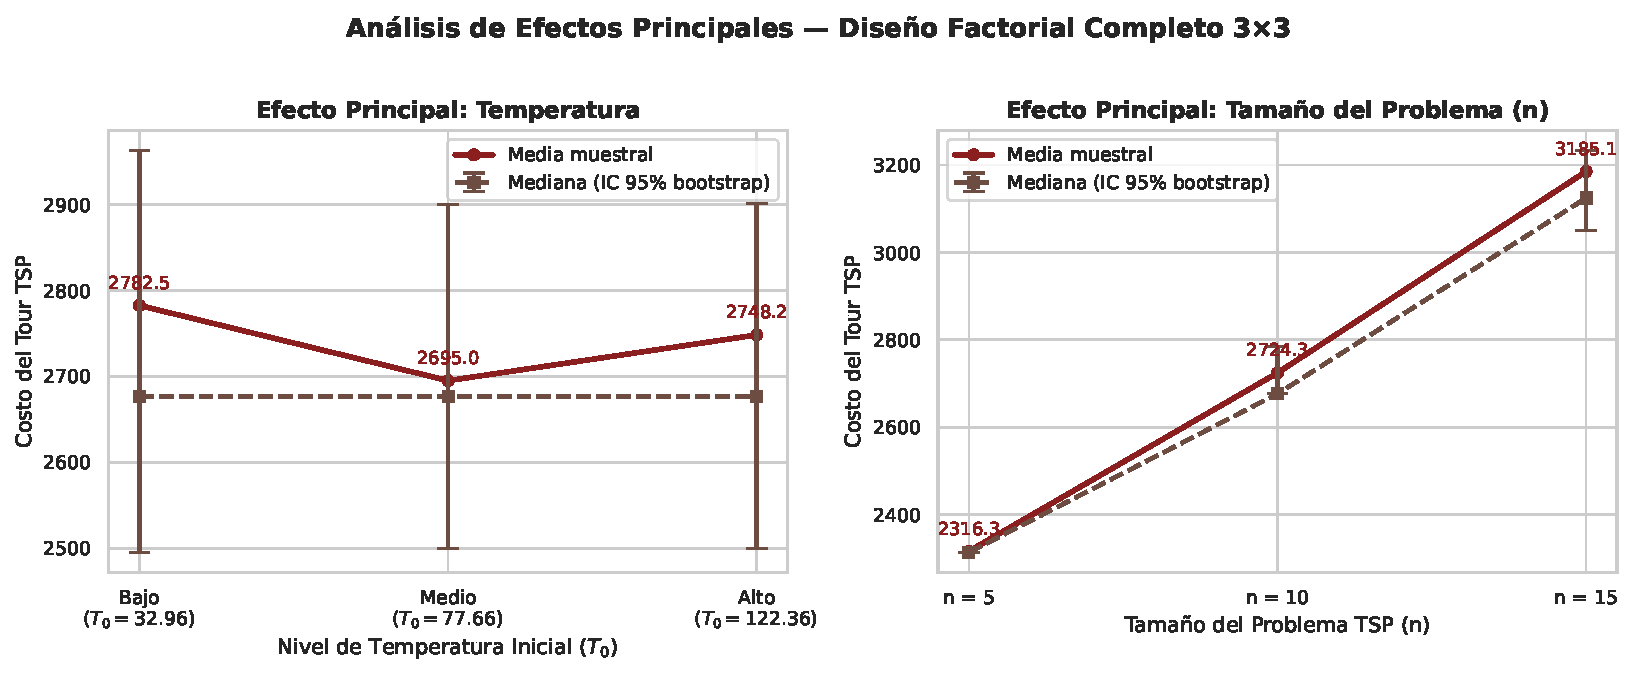
\includegraphics[width=0.98\textwidth]{main_effects.pdf}
    \caption{Gráfica de efectos principales para la temperatura inicial $T_0$ (izquierda) y el tamaño del problema TSP $n$ (derecha).}
    \label{fig:main_effects}
\end{figure}

La Figura~\ref{fig:interaction} evidencia la interacción Temperatura $\times$ Tamaño. En el panel derecho (incremento porcentual respecto al óptimo de cada bloque) se aprecia claramente el cruce y cambio de pendiente: para $n = 5$ el error crece ligeramente al subir la temperatura, para $n = 10$ las medianas coinciden en el óptimo global y las diferencias son marginales, mientras que para $n = 15$ se forma una pronunciada curva en ``U'' donde tanto $T_{\text{Bajo}}$ ($+10.02\%$ sobre la mejor mediana) como $T_{\text{Alto}}$ ($+4.63\%$) pierden desempeño respecto a $T_{\text{Medio}}$.

\begin{figure}[H]
    \centering
    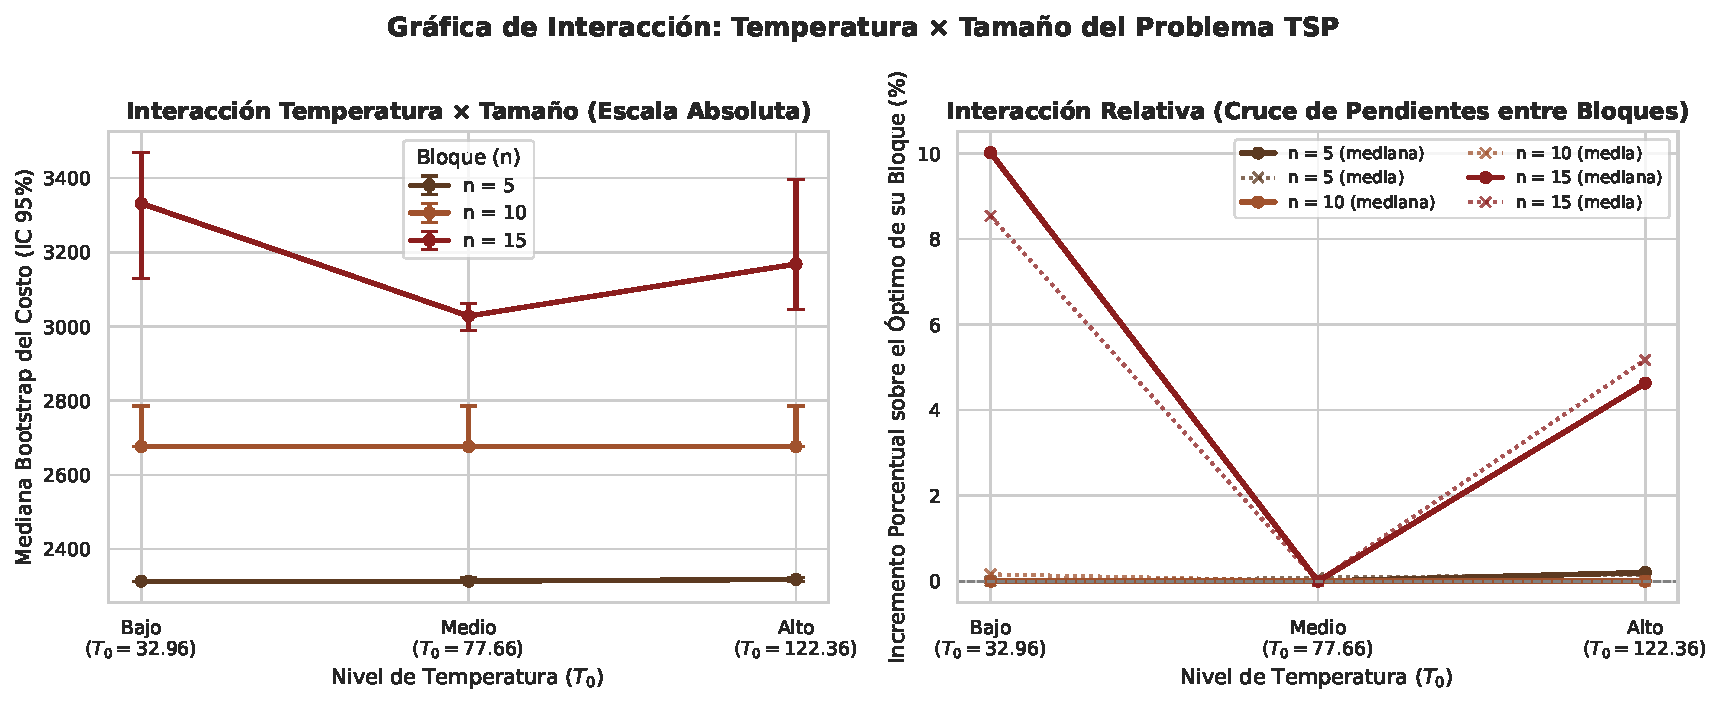
\includegraphics[width=0.98\textwidth]{interaction.pdf}
    \caption{Gráfica de interacción Temperatura $\times$ Tamaño en escala absoluta (izquierda) y relativa porcentual dentro de cada bloque (derecha).}
    \label{fig:interaction}
\end{figure}

Dado que los tres términos del ANOVA fueron significativos, se calcularon la mediana \textit{bootstrap} ($B = 10{,}000$ remuestreos con reemplazo) y su intervalo de confianza del 95\% por percentiles para los 9 puntos de diseño (Figura~\ref{fig:bootstrap}).

\begin{figure}[H]
    \centering
    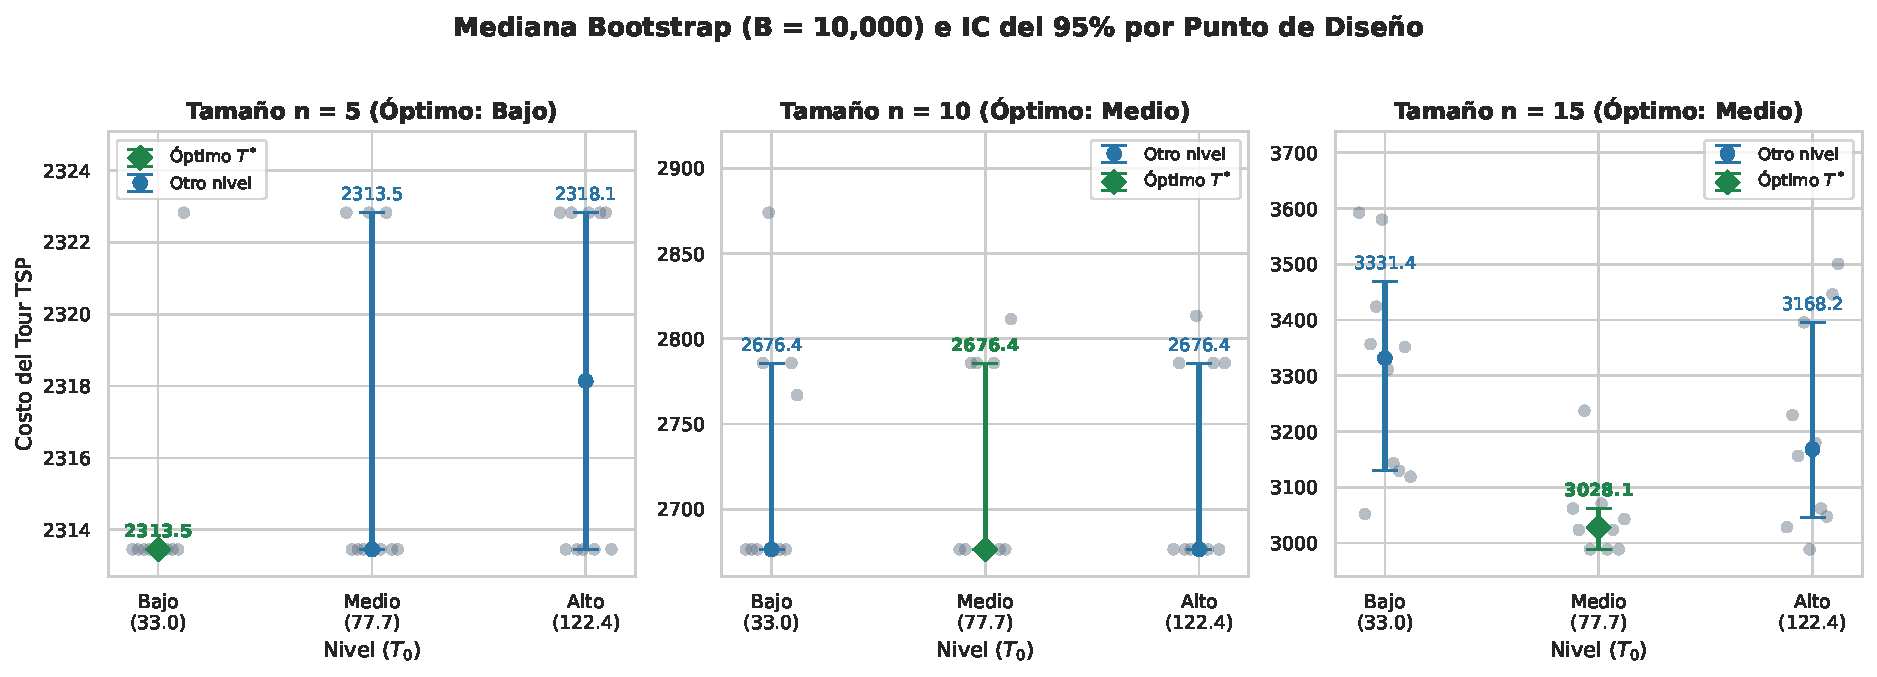
\includegraphics[width=0.98\textwidth]{bootstrap_intervals.pdf}
    \caption{Distribución de las 10 réplicas, mediana \textit{bootstrap} ($B = 10{,}000$) e IC 95\% para cada punto de diseño. En verde se resalta la temperatura óptima seleccionada por tamaño.}
    \label{fig:bootstrap}
\end{figure}

\section{Estimación Bootstrap y Tabla Resumen de Parámetros Óptimos}

El Cuadro~\ref{tab:bootstrap_all} detalla las estadísticas muestrales y \textit{bootstrap} para los 9 puntos de diseño, mientras que el Cuadro~\ref{tab:optimal_summary} resume la temperatura seleccionada como óptima para cada tamaño $n \in \{5, 10, 15\}$.

\begin{table}[H]
\centering
\caption{Resultados detallados por punto de diseño ($B = 10{,}000$ remuestreos \textit{bootstrap}, IC 95\%).}
\label{tab:bootstrap_all}
\begin{tabular}{@{}clrrrrrr@{}}
\toprule
\textbf{$n$} & \textbf{Nivel} & \textbf{$T_0$} & \textbf{Media} & \textbf{Desv. Est.} & \textbf{Mediana Boot.} & \textbf{IC 95\% Inf.} & \textbf{IC 95\% Sup.} \\
\midrule
5  & \textcolor{optgreen}{\textbf{Bajo*}}  & $32.96$  & $2314.39$ & $2.96$   & $\mathbf{2313.45}$ & $2313.45$ & $2313.45$ \\
5  & Medio                                 & $77.66$  & $2316.27$ & $4.53$   & $2313.45$          & $2313.45$ & $2322.83$ \\
5  & Alto                                  & $122.36$ & $2318.14$ & $4.94$   & $2318.14$          & $2313.45$ & $2322.83$ \\
\midrule
10 & Bajo                                  & $32.96$  & $2727.10$ & $71.04$  & $2676.45$          & $2676.45$ & $2785.73$ \\
10 & \textcolor{optgreen}{\textbf{Medio*}} & $77.66$  & $2722.74$ & $60.23$  & $\mathbf{2676.45}$ & $2676.45$ & $2785.73$ \\
10 & Alto                                  & $122.36$ & $2722.94$ & $60.56$  & $2676.45$          & $2676.45$ & $2785.73$ \\
\midrule
15 & Bajo                                  & $32.96$  & $3306.02$ & $192.23$ & $3331.42$          & $3129.73$ & $3468.36$ \\
15 & \textcolor{optgreen}{\textbf{Medio*}} & $77.66$  & $3045.93$ & $73.45$  & $\mathbf{3028.08}$ & $2988.68$ & $3061.99$ \\
15 & Alto                                  & $122.36$ & $3203.49$ & $185.20$ & $3168.24$          & $3045.20$ & $3395.72$ \\
\bottomrule
\end{tabular}
\end{table}

\begin{table}[H]
\centering
\caption{Tabla resumen de la temperatura inicial óptima ($T_0^*$) para cada tamaño del TSP.}
\label{tab:optimal_summary}
\begin{tabular}{@{}ccccc@{}}
\toprule
\textbf{Tamaño ($n$)} & \textbf{Nivel Óptimo} & \textbf{Temperatura $T_0^*$} & \textbf{Mediana Bootstrap} & \textbf{IC 95\% Bootstrap} \\
\midrule
$5$  & Bajo  & $32.9556$ & $2313.4535$ & $[2313.4535,\; 2313.4535]$ \\
$10$ & Medio & $77.6556$ & $2676.4468$ & $[2676.4468,\; 2785.7350]$ \\
$15$ & Medio & $77.6556$ & $3028.0827$ & $[2988.6778,\; 3061.9949]$ \\
\bottomrule
\end{tabular}
\end{table}

\section{Análisis y Respuestas a las Preguntas}

\subsection{¿Cuál fue el mejor parámetro para cada tamaño y cómo se llegó a esa conclusión?}
A partir de la significancia confirmada por el ANOVA de dos factores tanto para la temperatura ($p = 0.004062$) como para la interacción Temperatura $\times$ Tamaño ($p = 0.000411$), se evaluaron los intervalos \textit{bootstrap} dentro de cada bloque $n$:
\begin{itemize}
    \item \textbf{Para $n = 5$:} El óptimo fue el nivel \textbf{Bajo} ($T_0^* = 32.96$). Alcanzó la mediana exacta del óptimo global Held-Karp ($2313.45$) con un intervalo de confianza del 95\% colapsado en $[2313.45, 2313.45]$ (9 de 10 réplicas convergieron al óptimo) y la menor media muestral ($2314.39$, desviación $2.96$). En cambio, el nivel Alto ($122.36$) elevó la mediana a $2318.14$ debido a que, tras 18 épocas ($T_f = 12.24$), aún conserva agitación térmica residual.
    \item \textbf{Para $n = 10$:} Los tres niveles empataron en mediana \textit{bootstrap} en el óptimo exacto ($2676.45$, IC 95\% $[2676.45, 2785.73]$). Aplicando el criterio de desempate por menor costo medio y menor variabilidad entre réplicas, se seleccionó el nivel \textbf{Medio} ($T_0^* = 77.66$), que obtuvo la menor media muestral ($2722.74$) y la menor desviación estándar ($60.23$, frente a $71.04$ de Bajo).
    \item \textbf{Para $n = 15$:} El óptimo indiscutible fue el nivel \textbf{Medio} ($T_0^* = 77.66$), con mediana \textit{bootstrap} de $3028.08$ (a solo $1.32\%$ del óptimo exacto Held-Karp de $2988.68$) y un IC 95\% sumamente estrecho de $[2988.68, 3061.99]$. Nótese que este intervalo de confianza es \textbf{completamente disjunto} respecto al del nivel Bajo ($[3129.73, 3468.36]$, mediana $3331.42$), lo que prueba con más del 95\% de confianza que $T_0 = 77.66$ supera significativamente a $T_0 = 32.96$. Asimismo, Medio mejora sustancialmente la precisión y mediana frente a Alto ($3168.24$, IC $[3045.20, 3395.72]$).
\end{itemize}

\subsection{¿La temperatura óptima cambia con el tamaño del problema? ¿Hay una tendencia clara entre $n$ y $T^*$?}
\textbf{Sí, la temperatura óptima cambia con el tamaño $n$ y se observa una tendencia creciente en la energía térmica inicial requerida conforme aumenta $n$}, respaldada por la interacción altamente significativa del ANOVA ($F = 5.7310$, $p = 0.000411$):
\begin{enumerate}
    \item \textbf{De $n = 5$ a $n = 10, 15$, $T^*$ aumenta de $32.96$ (Bajo) a $77.66$ (Medio):} El espacio de tours no dirigidos crece de manera factorial como $(n-1)!/2$, pasando de apenas $12$ recorridos en $n = 5$ a $181{,}440$ en $n = 10$ y a $4.36 \times 10^{10}$ en $n = 15$. En $n = 5$ prácticamente no existen óptimos locales profundos para el operador 2-opt, por lo que una temperatura baja favorece una rápida explotación hacia el óptimo global sin introducir ruido térmico al final del enfriamiento.
    \item \textbf{Proliferación de mínimos locales en $n = 15$:} Al crecer $n$ a $15$, el paisaje de energía desarrolla múltiples óptimos locales subóptimos. Una temperatura baja ($T_0 = 32.96$) produce un congelamiento prematuro: el algoritmo rechaza casi de inmediato los movimientos $\Delta E > 0$ y queda atrapado en recorridos promedio un $10\%$ más costosos. Por ello, al aumentar $n$ se vuelve indispensable incrementar $T_0$ hacia el nivel Medio ($77.66$) para atravesar barreras de energía en las primeras épocas.
    \item \textbf{Límite superior térmico (equilibrio exploración--explotación):} Si bien $T^*$ tiende a subir con $n$, no crece de forma ilimitada bajo un presupuesto fijo de enfriamiento: en $n = 15$, elevar demasiado $T_0$ al nivel Alto ($122.36$) degrada nuevamente la solución ($3168.24$ vs.\ $3028.08$) porque la cadena termina las 18 épocas con temperatura residual alta ($T_f = 12.24$) sin consolidar la fase de explotación. En síntesis, $T^*$ muestra una tendencia ascendente con $n$ desde regímenes puramente explotativos (Bajo en $n=5$) hacia temperaturas intermedias balanceadas (Medio en $n=10, 15$).
\end{enumerate}

\end{document}
